Outra forma de construir soluções boas para o MCSP é utilizando meta-heurísticas, i.e., algoritmos de otimização que utilizam aleatorização em conjunto com busca local \cite[p.~4]{yang_nature-inspired_2010}. Antes de aplicar algum dos vários algoritmos conhecidos, no entanto, é necessário representar as instâncias do problema utilizando uma estrutura de dados eficiente e adequada para tais procedimentos. Encontrar uma boa representação para problemas complexos, como esse, é uma etapa desafiadora, mas que pode simplificar muito a resolução.

\begin{definition}
    Um \textbf{bloco} $S[a, b]$ de uma string $S$, com $1 \leq a \leq b \leq |S|$ é a substring de $S$ que inicia no índice $a$ e termina no índice $b$.
\end{definition}

Desenvolvemos uma representação na qual uma instância $(S, P)$ é dada por um grafo que contém as informações necessárias sobre da relação entre $S$ e $P$. Os vértices são os índices dos caracteres de $S$ e cada aresta entre dois caracteres representa um bloco entre eles e um outro bloco igual em $P$. Representações parecidas com essa já foram utilizadas para a aplicação de meta-heurísticas no MCSP de forma diferente da aqui apresentada \cite{ferdous_solving_2013}.

De forma mais formal, uma entrada $(S, P)$ do problema é representada pelo multigrafo $G_{S, P}(V, E, \phi)$, em que

\begin{itemize}
    \item $V = \{ 1, ..., |S| \}$
    \item $e_{s, p, k} \in E \iff S[s, s + k] = P[p, p + k] \text{ e } k \neq 0$
    \item $\phi(e_{s, p, k}) = (s, s + k)$
\end{itemize}

Note que cada par de bloco representado por uma aresta pode ser utilizado na construção de uma partição comum entre as strings. Arestas paralelas indicam que existe mais de um bloco em $P$ igual à substring formada pelos caracteres entre suas extremidades. Um exemplo da representação pode ser visto na \cref{fig:grafo}.

É importante ressaltar que blocos de tamanho unitário (apenas 1 caractere) não são considerados. Como as strings de entrada são balanceadas e os blocos dos pares são idênticos, ao partir de uma partição incompleta, podemos completá-la com todos os caracteres não contidos na partição como blocos unitários. Não considerar tais blocos reduz consideravelmente o número de arestas da representação, e consequentemente possibilita algoritmos mais eficientes.

\begin{figure}
    \centering
    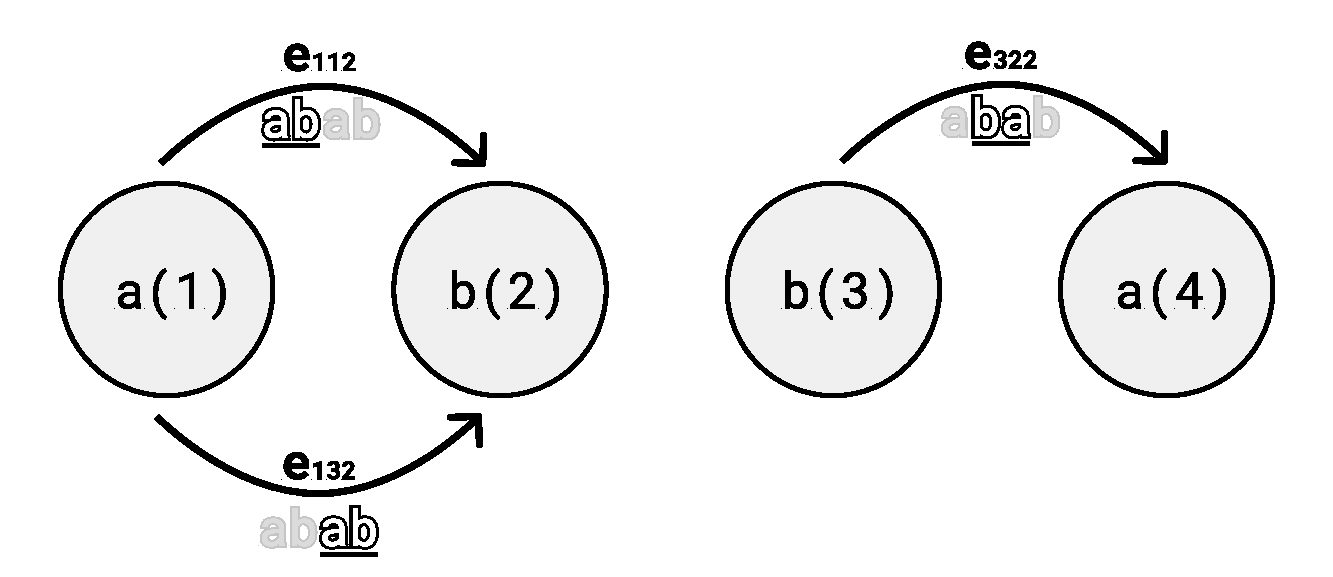
\includegraphics[width=0.6\textwidth]{images/grafo.pdf}
    \caption{Grafo representando a instância (\texttt{"abba"},~\texttt{"abab"}).}
    \label{fig:grafo}
    \todo[inline]{Trocar a figura}
\end{figure}

\subsection{Construindo partições}

    A partir de uma sequência ordenada das arestas da representação de uma instância do MCSP, podemos construir partições da seguinte forma: para cada aresta, na ordem dada, incluímos os dois blocos à partição se nenhum deles coincide com caracteres contidos em blocos que foram incluídos. Ao fim do processo, cria-se blocos unitários para todos os caracteres não contidos em um bloco. Dessa forma, uma permutação do conjunto de arestas do grafo representa uma única partição comum entre as strings de entrada do problema.
    
    É válido ressaltar duas propriedades dessa representação. Primeiramente, nem todas as possíveis partições possuem uma permutação correspondente, já que os blocos unitários são omitidos. Tais partições, no entanto, não são as mais interessantes para o MCSP, já que buscamos partições menores.

    Em segundo lugar, note que a partição formada por uma permutação das arestas não é única: podemos trocar de posição arestas vizinhas que não são utilizadas, de forma que o mesmo resultado é obtido.

\subsection{Aplicação da representação}

    Com a construção dessa representação, agora o MCSP se reduz a encontrar uma forma de ordenar as arestas de forma que a partição resultante seja a menor possível. Isso significa que o reduzimos a um problema de permutação. Algoritmos de otimização que atuam em um espaço de busca contínuo podem ser utilizados para esse tipo de problema aplicando um sistema de pesos que assumem valores reais \cite[p.~661]{marti_handbook_2018}. Relacionamos o vetor de arestas com um vetor de pesos de mesmo tamanho, de forma que a ordenação das arestas pelos valores dos pesos correspondentes forma a permutação correspondente àqueles valores. Como cada peso é uma componente no espaço de busca, podemos nos referir ao vetor de pesos também como posição (e à sua variação, como velocidade).
    